%
% This is a borrowed LaTeX template file for lecture notes for CS267,
% Applications of Parallel Computing, UCBerkeley EECS Department.
% Now being used for CMU's 10725 Fall 2012 Optimization course
% taught by Geoff Gordon and Ryan Tibshirani.  When preparing 
% LaTeX notes for this class, please use this template.
%
% To familiarize yourself with this template, the body contains
% some examples of its use.  Look them over.  Then you can
% run LaTeX on this file.  After you have LaTeXed this file then
% you can look over the result either by printing it out with
% dvips or using xdvi. "pdflatex template.tex" should also work.
%

\documentclass[twoside]{article}
\setlength{\oddsidemargin}{0.25 in}
\setlength{\evensidemargin}{-0.25 in}
\setlength{\topmargin}{-0.6 in}
\setlength{\textwidth}{6.5 in}
\setlength{\textheight}{8.5 in}
\setlength{\headsep}{0.75 in}
\setlength{\parindent}{0 in}
\setlength{\parskip}{0.1 in}

%
% ADD PACKAGES here:
%

\usepackage{amsmath,amsfonts,graphicx}

%
% The following commands set up the lecnum (lecture number)
% counter and make various numbering schemes work relative
% to the lecture number.
%
\newcounter{lecnum}
\renewcommand{\thepage}{\thelecnum-\arabic{page}}
\renewcommand{\thesection}{\thelecnum.\arabic{section}}
\renewcommand{\theequation}{\thelecnum.\arabic{equation}}
\renewcommand{\thefigure}{\thelecnum.\arabic{figure}}
\renewcommand{\thetable}{\thelecnum.\arabic{table}}

%
% The following macro is used to generate the header.
%
\newcommand{\lecture}[4]{
   \pagestyle{myheadings}
   \thispagestyle{plain}
   \newpage
   \setcounter{lecnum}{#1}
   \setcounter{page}{1}
   \noindent
   \begin{center}
   \framebox{
      \vbox{\vspace{2mm}
    \hbox to 6.28in { {\bf CS281: Advanced ML
	\hfill Fall 2017} }
       \vspace{4mm}
       \hbox to 6.28in { {\Large \hfill Lecture #1: #2  \hfill} }
       \vspace{2mm}
       \hbox to 6.28in { {\it Lecturer: #3 \hfill Scribes: #4} }
      \vspace{2mm}}
   }
   \end{center}
   \markboth{Lecture #1: #2}{Lecture #1: #2}

   {\bf Note}: {\it LaTeX template courtesy of UC Berkeley EECS dept.}
}
%
% Convention for citations is authors' initials followed by the year.
% For example, to cite a paper by Leighton and Maggs you would type
% \cite{LM89}, and to cite a paper by Strassen you would type \cite{S69}.
% (To avoid bibliography problems, for now we redefine the \cite command.)
% Also commands that create a suitable format for the reference list.
\renewcommand{\cite}[1]{[#1]}
\def\beginrefs{\begin{list}%
        {[\arabic{equation}]}{\usecounter{equation}
         \setlength{\leftmargin}{2.0truecm}\setlength{\labelsep}{0.4truecm}%
         \setlength{\labelwidth}{1.6truecm}}}
\def\endrefs{\end{list}}
\def\bibentry#1{\item[\hbox{[#1]}]}

%Use this command for a figure; it puts a figure in wherever you want it.
%usage: \fig{NUMBER}{SPACE-IN-INCHES}{CAPTION}
\newcommand{\fig}[3]{
			\vspace{#2}
			\begin{center}
			Figure \thelecnum.#1:~#3
			\end{center}
	}
% Use these for theorems, lemmas, proofs, etc.
\newtheorem{theorem}{Theorem}[lecnum]
\newtheorem{lemma}[theorem]{Lemma}
\newtheorem{proposition}[theorem]{Proposition}
\newtheorem{claim}[theorem]{Claim}
\newtheorem{corollary}[theorem]{Corollary}
\newtheorem{definition}[theorem]{Definition}
\newenvironment{proof}{{\bf Proof:}}{\hfill\rule{2mm}{2mm}}

% **** IF YOU WANT TO DEFINE ADDITIONAL MACROS FOR YOURSELF, PUT THEM HERE:

\newcommand\E{\mathbb{E}}

\begin{document}
%FILL IN THE RIGHT INFO.
%\lecture{**LECTURE-NUMBER**}{**DATE**}{**LECTURER**}{**SCRIBE**}
\lecture{1}{September 6}{Sasha Rush}{Anna Sophie Hilgard}
%\footnotetext{These notes are partially based on those of Nigel Mansell.}

% **** YOUR NOTES GO HERE:

% Some general latex examples and examples making use of the
% macros follow.  
%**** IN GENERAL, BE BRIEF. LONG SCRIBE NOTES, NO MATTER HOW WELL WRITTEN,
%**** ARE NEVER READ BY ANYBODY.

\section{Discrete Models} % Don't be this informal in your notes!

\begin{itemize}
\item Take values from a countable set, e.g. \{0,1\}, \{cold, flu, asthma\}
\item We will use simple discrete models to develop our tactics such as marginalization and conditioning. Today: coins
\end{itemize}

\section{Bernoulli model with $p(heads) = \theta$} 

\subsection{Easy Prior}
Assume we know the coin came from one of 3 unknown manufacturers (Later, we'll have mixture model estimation, but for now assume these probabilities come from an oracle.\\
$\theta = 0.4$ with probability .1\\
$\theta = 0.5$ with probability .8\\
$\theta = 0.6$ with probability .1

$p(\theta) = 0.1 \cdot \delta(\theta = 0.4)  + 0.8 \cdot \delta(\theta = 0.5) + 0.1 \cdot \delta(\theta = 0.6)$


\subsection{Likelihood}
Likelihood: $p(data|parameters)$

Ex: $p(coin\_flips|\theta) = \textrm{Bin}(N_1 | N, \theta) = {N \choose N_1} \theta^{N_1} (1-\theta)^{N-N_1}$\\
Where $N = N_0 + N_1 =$ number of flips\\
Note that the last term, the ``score", is the only term that depends on theta

\section{Inference}
Inference 1: $p(\theta|x)$ ($x = N_0, N_1$)

\subsection{Maximum Likelihood Estimation (MLE)}
$\theta_{MLE} = \textrm{argmax}_{\theta} \; p(N_0,N_1 | \theta) = \textrm{argmax}_{\theta}  \;\textrm{log}\left[p(N_0,N_1 | \theta)\right]$

$\theta_{MLE} = \textrm{argmax}_{\theta} \;\textrm{log}{N \choose N_1} + N_1 \textrm{log} \theta + N_0  \textrm{log} (1-\theta)$

Because the first term is not a function of $\theta$, we can ignore it.

$\frac{d}{d\theta} = \frac{N_1}{\theta} + \frac{N_0}{1-\theta} \cdot ( -1)  \rightarrow \theta_{MLE} = \frac{N_1}{N_0 + N_1}$

\begin{itemize}
\item Note that Inference != Decision Making. If we asked you to make a bet on the coin, based on this you could either
\begin{enumerate}
\item Always take heads if $\theta > .5$. In this case, $p(win) = \theta$
\item Take heads with probability = $\theta$. In this case, $p(win) = \theta^2 + (1-\theta)^2$ [p(is heads) * p(choose heads) + ...]
\end{enumerate}
For $\theta = .6$, the win probabilities are .6 and .52, respectively. 
\end{itemize}

\subsection{Maximizing the Posterior (MAP)}
Bayes Rule : $p(\theta|data) \propto p(data|\theta) p(\theta)$
\begin{itemize}
\item Posterior: $p(\theta | x)$
\item Likelihood: $p(x | \theta)$
\item Prior: $p(\theta)$
\end{itemize}
$\theta_{MAP} = \textrm{argmax}_{\theta} \; p(\theta | x) = \textrm{argmax}_{\theta}  \;\textrm{log}\left[p(x | \theta) p(\theta)\right]$\\

Ex:\\
$p(\theta=0.4|N_0,N_1) \propto {N \choose N_1} (.4)^{N_1}(1-.4)^{N_0} (0.1)$

$p(\theta=0.45|N_0,N_1) = 0 $ (Due to the sparsity of the prior)\\

MAP = MLE when we have a uniform prior

\subsection{Full Posterior}

\begin{itemize}
\item Partition/Marginal: $p(N_0,N_1) = \int_\theta p(N_0,N_1,\theta)$. Note this is evil and hard to compute
\end{itemize}
$p(\theta|N_0,N_1) = \frac{p(x|\theta) p(\theta)}{p(N_0,N_1)}$

\subsection{Beta Prior}

Beta Distribution: $p(\theta|\alpha_0,\alpha_1) = \frac{\Gamma(\alpha_0 + \alpha_1)}{\Gamma(\alpha_0)\Gamma(\alpha_1)} \theta^{\alpha_1-1} (1-\theta)^{\alpha_0-1}$ 

From the image of the beta function for different parameters, we can see that it can ether be balanced, humped to one side, or tend toward infinity on one side or the other.
\begin{figure}
\centering
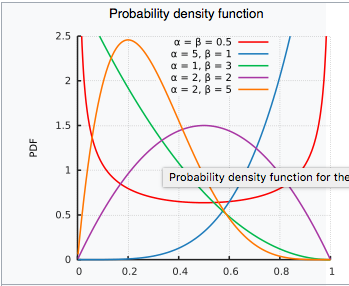
\includegraphics[width=0.5\textwidth]{beta}
\caption{Beta Params}
\end{figure}

With a beta prior:  $p(\theta|N_0,N_1) = \frac{\Gamma(\alpha_0 + \alpha_1)}{\Gamma(\alpha_0)\Gamma(\alpha_1)} \theta^{\alpha_1-1} (1-\theta)^{\alpha_0-1} \theta^{N_1}(1-\theta)^{N_0} \cdot \textrm{(some constant normalizer that does not depend on } \theta) $

The key insight is that we get additive terms in the exponent and the resulting distribution looks like another beta. The prior ``counts'' (pseudocounts) from the hyperparameters can be interpreted as counts we have beforehand

$p(\theta|N_0,N_1) = \frac{\Gamma(\alpha_0 + \alpha_1)}{\Gamma(\alpha_0)\Gamma(\alpha_1)} \theta^{N_1 + \alpha_1-1} (1-\theta)^{N_0 + \alpha_0-1} \cdot \textrm{(constant)}$ 

To make this distribution sum to 1, use the known beta normalizer

$p(\theta|N_0,N_1) = \frac{\Gamma(\alpha_0 + \alpha_1 + N_0 + N_1)}{\Gamma(\alpha_0)\Gamma(\alpha_1)\Gamma(N_0)\Gamma(N_1)} \theta^{N_1 + \alpha_1-1} (1-\theta)^{N_0 + \alpha_0-1} $ 

$p(\theta|N_0,N_1) \sim \textrm{Beta}(\theta | N_0 + \alpha_0, N_1 + \alpha_1)$ is the posterior distribution.

\begin{itemize}
\item The mode of the Beta gives us back the MAP, but we additionally now have information about the shape.
\item What does the prior that tends to infinity at 1 imply? That in the absence of other information, the coin is definitely heads. 
\end{itemize}

\subsection{Predictive Distribution}

$p(\hat{x}| N_0, N_1) = \int_\theta p(x|\theta, N_0, N_1) p(\theta | N_0, N_1) d\theta$

$p(\hat{x}| N_0, N_1) = \int_\theta \theta p(\theta | N_0, N_1) d\theta$

$p(\hat{x}| N_0, N_1) = \E_{\theta \sim p(\theta|N_0, N_1)} \theta$ (The expectation under the posterior of $\theta$. This is the mean of the Beta distribution. Feel free to prove it as an exercise!)

\subsection{Normalizing Term / Marginal (Likelihood)}
$p(N_0, N_1) = \int_\theta p(x_1, \hdots x_n | \theta) p(\theta) d\theta$ \\
$p(N_0, N_1) = \int_\theta \frac{\Gamma( \alpha_1 +  \alpha_1)}{\Gamma(\alpha_0)\Gamma(\alpha_1)} \theta^{\alpha_1 + N_1 -1} (1-\theta)^{\alpha_0+N_0-1} $

The first term can be moved outside, as it does not depend on $\theta$. Then we know what the integral of the rest should be because we know how to make the distribution sum to 1.

$p(N_0, N_1) = \frac{\Gamma( \alpha_1 +  \alpha_1)}{\Gamma(\alpha_0)\Gamma(\alpha_1)} \frac{\Gamma(N_0 + \alpha_0)\Gamma(N_1 + \alpha_1}{\Gamma(N_0 + N_1 + \alpha_0 + \alpha_1}$

\section{Extensions on the Coin Flip Model: Super Coins}
\begin{itemize}
\item Many coins and they're correlated (Models of binary data)
\item Many-sided coins aka dice (Models of categorical data)
\end{itemize}

\subsection{Bernoulli}
$\textrm{Ber}(x|\theta) = \theta^{x}(1-\theta)^x$
\subsection{Categorical}
$\textrm{Cat}(x|\theta) = \prod_k\theta_k^{x_k}$
\subsection{Multinomial}
$\textrm{Multi}(x|\theta) = \frac{(\sum x_k) !}{\prod_k x_k!}\prod_k\theta_k^{x_k}$
\subsection{Dirichlet}
$\textrm{Dir}(x|\alpha) = \frac{\Gamma(\sum \alpha_k)}{\prod \Gamma(\alpha_k)}\prod_k\theta_k^{\alpha_k-1}$
% **** THIS ENDS THE EXAMPLES. DON'T DELETE THE FOLLOWING LINE:

\section{See Beta.ipynb}
\end{document}


